%
% File acl2020.tex
%
%% Based on the style files for ACL 2020, which were
%% Based on the style files for ACL 2018, NAACL 2018/19, which were
%% Based on the style files for ACL-2015, with some improvements
%%  taken from the NAACL-2016 style
%% Based on the style files for ACL-2014, which were, in turn,
%% based on ACL-2013, ACL-2012, ACL-2011, ACL-2010, ACL-IJCNLP-2009,
%% EACL-2009, IJCNLP-2008...
%% Based on the style files for EACL 2006 by 
%%e.agirre@ehu.es or Sergi.Balari@uab.es
%% and that of ACL 08 by Joakim Nivre and Noah Smith

\documentclass[11pt,a4paper]{article}
\usepackage[hyperref]{acl2020}
\usepackage{amsmath}
\usepackage{times}
\usepackage{subfigure}
\usepackage{latexsym}
\renewcommand{\UrlFont}{\ttfamily\small}
% \hypersetup{draft=true}

% This is not strictly necessary, and may be commented out,
% but it will improve the layout of the manuscript,
% and will typically save some space.
\usepackage{microtype}

% TODO(sst): enter aclpaperid here
%\aclfinalcopy % Uncomment this line for the final submission
%\def\aclpaperid{***} %  Enter the acl Paper ID here

%\setlength\titlebox{5cm}
% You can expand the titlebox if you need extra space
% to show all the authors. Please do not make the titlebox
% smaller than 5cm (the original size); we will check this
% in the camera-ready version and ask you to change it back.

\title{The spontaneous emergence of discrete and compositional messages
	\\ \nbSST{(1) Thoughts on the title? (2) It's hidden on submission, but we need to decide author order as well.}
}

% TODO(sst): anonymous, so doesn't matter now, but: is this the right author order?
\author{Nur Lan \\
  Computational Linguistics Lab \\
  Tel Aviv University \\
  \texttt{nurlan@mail.tau.ac.il} \\\And
  Shane Steinert-Threlkeld \\
  Department of Linguistics \\
  University of Washington \\
  \texttt{shanest@uw.edu} \\\And
  Emmanuel Chemla \\
  Laboratoire de Sciences Cognitives et Psycholinguistique \\
  Ecole Normale Sup\'erieure \\
  \texttt{chemla@ens.fr}}

\date{}

\usepackage{multicol}  % for big figures
\usepackage{amsmath}
\usepackage{graphicx}

\DeclareMathOperator*{\argmax}{arg\,max}
\DeclareMathOperator*{\argmin}{arg\,min}

\newcommand{\changeEC}[2]{{\leavevmode\color{gray}{\scriptsize{#1}}~\color{blue}#2}}
\newcommand{\nbEC}[1]{{\leavevmode\color{blue}{\scriptsize#1}}}
\newcommand{\addEC}[1]{{\leavevmode\color{blue}#1}}

\newcommand{\changeNL}[2]{{\leavevmode\color{gray}{\scriptsize{#1}}~\color{red}#2}}
\newcommand{\nbNL}[1]{{\leavevmode\color{red}{\scriptsize#1}}}
\newcommand{\addNL}[1]{{\leavevmode\color{red}#1}}

\newcommand{\changeSST}[2]{{\leavevmode\color{gray}{\scriptsize{#1}}~\color{violet}#2}}
\newcommand{\nbSST}[1]{{\leavevmode\color{violet}{\scriptsize#1}}}
\newcommand{\addSST}[1]{{\leavevmode\color{violet}#1}}


\begin{document}

\maketitle
% TODO(sst): short [4] or long [8] paper?

\begin{abstract}
	\nbSST{To be written.}
\end{abstract}

\section{Introduction}

In a signalling game, artificial agents learn to communicate to achieve a common goal: a sender sees some piece of information and produces a message, this message is then sent to a receiver that must take some action \citep{Lewis1969, Skyrms2010}. If the action is coherent with the sender's initial piece of information, the whole communication stream ---the choice of the message and its interpretation--- is reinforced. 
For instance, in a referential game, sender and receiver see a set of objects, and the sender knows which of these the receiver must pick; the sender thus sends a message to the receiver, who must interpret it to pick up the right object \citep{Lazaridou2017, Lazaridou2018, Havrylov2017, Chaabouni2019a}.
%For instance, in a referential game, sender and receiver see a set of objects, and the sender must send a message to the receiver, so that the receiver can pick up the right object, as determined in advance for the sender, but unbeknownst to the receiver \citep{Lazaridou2017, Lazaridou2018, Havrylov2017, Chaabouni2019a}.

This setting has been used to study the factors influencing the emergence of various fundamental properties of natural language, such as \emph{compositionality} \citep{Kirby2015, Franke2016, SteinertThrelkeld2016, Mordatch2018, Lazaridou2018, Choi2018}.
In this paper, we add focus on two other so-called `design features' of natural language \citep{Hockett1960}: 
\emph{discreteness} (i.e.~words form clusters in acoustic space), 
and \emph{displacement} (i.e.~efficient communication can occur about objects and facts beyond the immediate context of the conversation).

From an implementation point of view, we follow the recent literature which has shown that a signalling game is essentially an autoencoder setting, with the encoder playing the role of the sender, and the decoder the role of the receiver. In this literature, however, the discreteness of the communication protocol is assumed, since the autoencoders use a (normally sequential and) discrete latent space \citep{Havrylov2017, Chaabouni2019a, Kharitonov2019}.  


Our main contribution is a generalization of the current implementation of signalling games as autoencoders, called Function Games. Our implementation covers a broader variety of signalling games, and it crucially incorporates the possibility of displacement and no \emph{a priori} assumption of discreteness. In this setting we propose new analyses for the degree of emergent discreteness, compositionality and displacement. Our main result is that under appropriate conditions, discreteness emerges spontaneously, that is, if the latent space is thought about as a continuous acoustic space, then trained messages form coherent clusters, just like regular words do.

In addition to contributing to our understanding of the emergence of communication protocols with features like natural language, these results have a technical significance: by using a fundamentally continuous communication protocol, with discreteness emerging, we can train end-to-end using standard backpropagation techniques, instead of reinforcement learning algorithms like REINFORCE and its refinements \citep{Williams1992, Schulman2015, Mnih2016}, which often have high variance and are difficult to use in practice.


%Our main contributions are:
%\begin{itemize}
%	\item A generalization of reference games called Function Games, with a natural incorporation of displacement.
%	\item An analysis of clusters in continuous latent space as discrete symbols.
%	\item Probes for compositional structure in the new symbol space.
%\end{itemize}
%
%In particular, we view signaling games as a kind of auto-encoder, with the continuous latent space being the communication protocol.  Under certain conditions, this space becomes discrete, with clusters that function in many ways like the symbols traditionally used in other studies.
%
%In addition to contributing to our understanding of the emergence of communication protocols with features like natural language, these results have a technical significance: by using a fundamentally continuous communication protocol, with discreteness emerging, we can train end-to-end using standard backpropagation techniques, instead of reinforcement learning algorithms like REINFORCE and its refinements \citep{Williams1992, Schulman2015, Mnih2016}, which often have high variance and are difficult to use in practice.
%
%\nbSST{Notes on introduction: I'm not sure how much to play up the auto-encoder thing or not; and I added in a reference to Hockett as a hook. These lists of ``contributions'' are not my favorite stylistically, but they seem to be the norm in this literature.  It's also common to have a ``Related Work'' section; but we're tight on space.  What do people think?}

\section{Related Work}

%Other papers have observed that reference games are analogous to autoencoders, albeit with a (normally sequential and) discrete latent space \citep{Havrylov2017, Chaabouni2019a, Kharitonov2019}.  All of these papers, however, assume the discreteness of the communication protocol.

A related line of work attempts to avoid the difficulties of reinforcement learning---which introduces stochastic nodes into a computation graph---by reparameterization and/or non-stochastic estimators \citep{Bengio2013, Schulman2015}.  In the emergent communication case, where the stochastic nodes are discrete (e.g.\ sampling a message from a sender distribution), the Gumbel-Softmax estimator has become increasingly popular \citep{Jang2017, Maddison2017}.  

This work enables standard back-propagation to be used for training by optimizing approximations to the true reinforcement learning signal.  By contrast, by taking the auto-encoder analogy seriously, we do not approximate the discrete RL learning signal, but rather ask under what conditions discreteness will emerge. \nbSST{Probably can be worded better.}

\section{Function Games}

We here introduce a general communication game setting, which we call Function Games.  Our games contain three basic components: (i) a set of contexts $C$, (ii) a set of actions $A$, (iii) a family of functions $F$, from contexts to actions.  One play of a Function Game game runs as follows:
\begin{enumerate}
	\item Nature chooses $f \in F$ and a context $c \in C$.
	\item Sender sees the context $c$ and $f$.
	\item Sender sends a message $m$ to Receiver.
	\item Receiver sees \emph{a possibly different} context $c'$ and the message $m$ and chooses an action $a'$.
	\item Both are `rewarded' iff $a' = f(c')$.
\end{enumerate}
Abstractly, the function $f$ represents some piece of knowledge available directly only to Sender, and which determines what action is appropriate in any given context. Two concrete interpretations will help illustrate the variety of communication protocols and goals that this framework encompasses.
%Two concrete interpretations will be helpful in illustrating the various components.

\noindent \textbf{Generalized referential games.}  A reference game is one in which Sender tries to get Receiver to pick the correct object out of a given set \citep{Skyrms2010, Lazaridou2017, Lazaridou2018, Havrylov2017, Chaabouni2019a}.  Here, contexts are sets of objects (i.e.\ an $m \times n$ matrix, with $m$ objects represented by $n$ features).  Normally (though we will drop this assumption later), $c' = \texttt{shuffled}(c)$: Sender and Receiver see the same objects, but in a different arrangement. Actions are the objects, and the functions $f \in F$ are \emph{choice functions}: $f(c) \in c$ for every context $c$.

\noindent \textbf{Belief update games.} Contexts can represent the (possibly different) belief states of the agents. `Actions' can represent updated belief states ($A = C$), the different functions in $F$ then representing how to update an agent's beliefs in the light of learning a particular piece of information (passed directly to Sender, and only through the message to Receiver). 
\nbSST{What should we cite here? Something from dynamic semantics?}

%\noindent \textbf{Belief update games.} Contexts can represent the (possibly different) belief states of the agents. Letting $A = C$, the functions can be seen as `belief update' functions, representing e.g.\ how to update an agent's beliefs in the light of learning a new piece of information (passed only through the message, as far as Receiver is concerned). 

\section{Experiment}

Because we are interested in the simultaneous emergence both of discrete signals and of compositional messages, we use a Function Game called the Extremity Game designed to incentivize and test rich compositionality \citep{Steinert-Threlkeld2019}. In this game, it is natural to think of the $n$ dimensions of the objects as gradable properties, e.g., size and darkness, so that a 2D object is determined by a given size and shade of gray. For the functions, we set $F = \left\{ \argmin_i , \argmax_i : 0 \leq i < n \right\}$ and, hopefully, the emerging language should contain messages like `(pick the) \textsc{most} + \textsc{big}', `\textsc{least} + \textsc{dark}', etc.


%Because we are interested in the simultaneous emergence both of discrete signals and of compositional messages, we use a Function Game called the Extremity Game designed to incentivize and test compositionality \citep{Steinert-Threlkeld2019}. This is a generalized referential game, where objects are represented as $n$-dimensional vectors, with each value corresponding to the degree to which it has a gradable property.  For instance, objects could be shaded circles, with two values, one for their diameter and one for their darkness.  For the functions, we set $F = \left\{ \argmin_i , \argmax_i : 0 \leq i < n \right\}$.  These may incentivize the emergence of communication protocols with messages like `small + EST' and `dark + EST'.

%This is a generalized referential game, where objects are represented as $n$-dimensional vectors, with each value corresponding to the degree to which it has a gradable property.  For instance, objects could be shaded circles, with two values, one for their diameter and one for their darkness.  For the functions, we set $F = \left\{ \argmin_i , \argmax_i : 0 \leq i < n \right\}$.  These may incentivize the emergence of communication protocols with messages like `small + EST' and `dark + EST'.

\nbSST{cite my forthcoming philosophy of science paper instead? pre-print is only on my website, so URL would be sort of de-anonymizing}

\subsection{Model}

Our model resembles an encoder-decoder architecture, with the Sender encoding the context/target pair into a message, and the Receiver decoding the message (together with its context $c'$) into an action.  Both the encoder and decoder are multi-layer perceptrons with two hidden layers of size 64 and rectified linear activation (ReLU) \citep{Nair2010, Glorot2011}. A smaller, intermediate layer without an activation function bridges the encoder and decoder and represents the transformation of the input information to messages. Figure~\ref{fig:model} depicts this architecture.

\begin{figure}[ht]
	\centering
	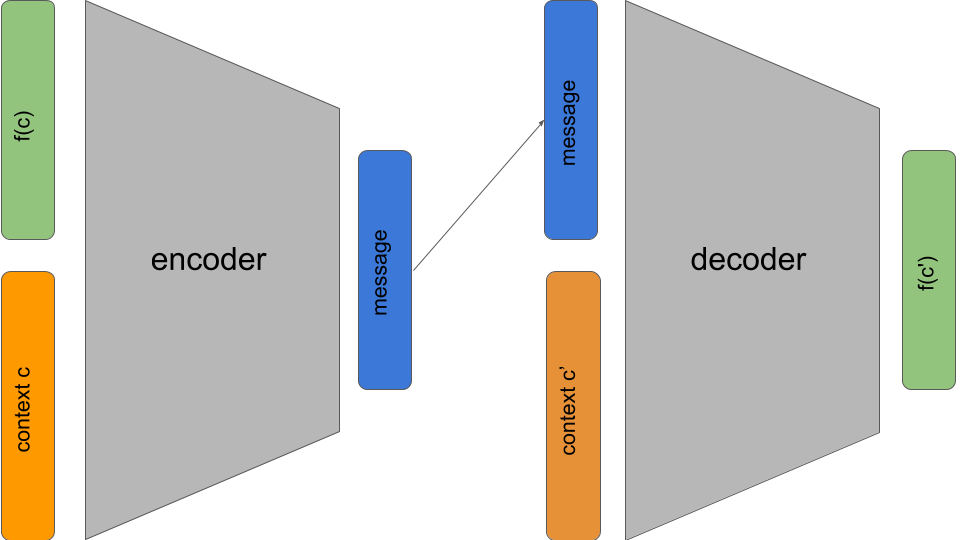
\includegraphics[width=\columnwidth]{figures/model_figure.png}
	\caption{Model architecture caption \nbSST{Do we really need this? It isn't super informative and might use too much space. I can also do something in TikZ if we think it's important and that this one is ugly.}}
	\label{fig:model}
\end{figure}

\subsection{Game Parameters}

We manipulated the following parameters:
%In our experiments, we manipulated the following parameters of the Extremity Game:
\begin{itemize}
	\item Context identity. 
	In the \emph{shared} setting, Receiver sees a shuffled version of Sender's context ($c' = \texttt{shuffled}(c)$). In the \emph{non-shared} setting, Receiver's context $c'$ is entirely distinct from Sender's. This forces displacement and may incentivize compositional messages, since Sender cannot rely on the raw properties of the target object in communication.

	\item Context strictness. 
	In \emph{strict} contexts, there is a one-to-one (and onto) correspondence between $F$ and \changeEC{$A = C$}{$A$}.%
\footnote{These are the contexts used in the original Extremity Game from \cite{Steinert-Threlkeld2019}. \nbEC{Drop if we need space? Or incorporate in text with 3 words, like `As in the original Extremity Game from \cite{Steinert-Threlkeld2019}'?}}
In \emph{non-strict} contexts, an object may be the $\argmax$ or $\argmin$ of several dimensions, or of no dimension.
%	In \emph{strict} contexts, every object is the $\argmax$ or $\argmin$ of exactly one dimension.  This means that there is a one-to-one (and onto) correspondence between $F$ and \changeEC{$A = C$}{$A$}.\footnote{These are the contexts used in \cite{Steinert-Threlkeld2019}.}  In \emph{non-strict} contexts, no such restriction is imposed.

\end{itemize}
In all experiments, the latent space (message) dimension was always 2,%
\footnote{The model also performs well with messages of size 1, not reported here. Using messages of size 2 makes it easier to inspect the latent space using 2-D visualization.}
and objects had 5 dimensions. Strict contexts therefore contained 10 objects, while non-strict contexts could contain 5, 10, or 15 objects.

\subsection{Training Details}

By using a continuous latent space, the entire model, including the communication channel, is differentiable and so can be trained end-to-end using backpropagation to compute gradients.
\nbEC{We can drop the previous sentence if we need space.}
We used the Adam optimizer \citep{Kingma2015} with learning rate 0.001, $\beta_1 = 0.9$, and $\beta_2 = 0.999$. The model was trained for 5,000 epochs by feeding the network with mini-batches of 64 contexts concatenated with one-hot function selectors. The network's loss is taken as the MSE between the target object $f(c')$ and the object generated by the Receiver. For each setting of the above parameters, we ran 20 trials with different random seeds.

Code and data will be made available once the paper can be de-anonymized. 

\section{Results}

We measure the communicative success of the network by calculating the accuracy of recovering the correct object from $c'$. The Receiver's prediction is considered correct if its output is closest to $f(c')$ than to all other objects in $c'$. The recovery accuracy of the different settings is reported in Table~\ref{tab:object_prediction_accuracy}. While the network handles well the $c \neq c'$ setting (\textit{unshared context}), the model struggles with non-strict contexts. Note that although accuracy is not $100\%$, it is still well above chance, since e.g. for a context of 10 objects random guessing will yield an expected accuracy of $10\%$. Table~\ref{tab:prediction_trained_untrained} shows the mean loss and recovery accuracy for a network before and after training. The randomly-initialized network's accuracy is at the expected chance level for a 10-object setting.

\begin{table}[]
\begin{tabular}{l|c|c}
\hline
                       & \textbf{Trained} & \textbf{Untrained} \\ \hline
\textbf{\begin{tabular}[c]{@{}l@{}}Accuracy\end{tabular}}  & 63.78$\%\pm 0.02$  & 9.92$\%\pm 0.01$      \\\hline
\textbf{\begin{tabular}[c]{@{}l@{}}Loss (MSE)\end{tabular}}    & $0.04\pm 0.00$  & $0.35\pm 0.03$      \\\hline
\end{tabular}
\caption{Mean object recovery accuracy and prediction loss before and after training, for objects of size 5 in a shared, strict context setting (10 objects per context).}\label{tab:prediction_trained_untrained}
\end{table}


\begin{table}[]
\begin{tabular}{l|c|c}
\hline
                       & \textbf{Shared} & \textbf{Non-shared} \\ \hline
\textbf{\begin{tabular}[c]{@{}l@{}}Strict \\ context \end{tabular}}                 & $63.78\%\pm 1.63$  & $60.22\%\pm 1.56$      \\\hline
\textbf{\begin{tabular}[c]{@{}l@{}}Non-strict, \\ 5 objects\end{tabular}}  & $49.37\%\pm 1.67$  & $43.55\%\pm 1.69$      \\\hline
\textbf{\begin{tabular}[c]{@{}l@{}}Non-strict, \\ 10 objects\end{tabular}} & $33.06\%\pm 1.47$  & $31.89\%\pm 1.63$      \\\hline
\textbf{\begin{tabular}[c]{@{}l@{}}Non-strict, \\ 15 objects\end{tabular}} & $27.58\%\pm 1.30$  & $27.95\%\pm 1.24$      \\ \hline
\end{tabular}
\caption{Object recovery accuracy for the different model settings.}\label{tab:object_prediction_accuracy}
\end{table}


\subsection{Discrete signals}

\begin{figure*}[ht]
  \centering
  Commented out the actual figures because I can't compile without them.
  \subfigure[]{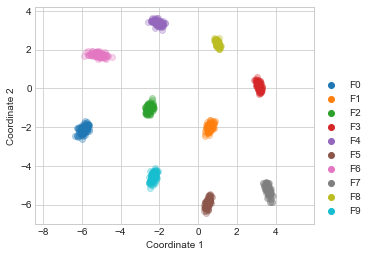
\includegraphics[scale=0.55]{./figures/messages_o5_shared_strict_trained.png}}\hspace{1cm}
  \subfigure[]{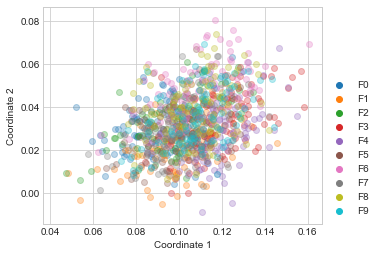
\includegraphics[scale=0.55]{./figures/messages_o5_untrained.png}}
  \caption{(a) Messages sampled from latent space of a trained network, for objects of size 5 and contexts of 10 objects. (b) Messages sampled from an untrained network. Colors represent the $f_i \in F$ input part of the Sender.}
 \label{fig:messages}
\end{figure*}

The model's ability to discretize the communication is measured by inspecting the information generated by the intermediate layer. Figure~\ref{fig:messages} depicts message vectors sampled from this layer. The same is depicted for an untrained network with randomized weights, where the messages are not yet clustered. 

We make the discretization measure concrete by calculating the F1 score between the cluster labels for transmitted messages and the target functions for which they were generated. For this, an unsupervized clustering algorithm is first applied to the message vectors, giving an expected number of clusters (DBSCAN, \citealp{ester_density-based_1996}, with $\epsilon = 0.5$). The cluster labels are then matched with the respective function labels by taking the most common function in each cluster. If message clusters are well separated from one another, the labeling will have less to no confusion and an F1 score closer to~$1$. The F1 scores for the different model settings are given in Table~\ref{tab:f1_scores}. The model reached near-optimal clusterization measures for both shared and non-shared contexts, and for both strict and non-strict contexts. 


\begin{table}[]
\begin{tabular}{l|c|c}
\hline
                       & \textbf{Shared} & \textbf{Non-shared} \\ \hline
\textbf{\begin{tabular}[c]{@{}l@{}}Strict \\ context \end{tabular}}                 & $1.00\pm 0.00$  & $0.90\pm 0.09$      \\\hline
\textbf{\begin{tabular}[c]{@{}l@{}}Non-strict, \\ 5 objects\end{tabular}}  & $0.99\pm 0.02$  & $0.54\pm 0.15$      \\\hline
\textbf{\begin{tabular}[c]{@{}l@{}}Non-strict, \\ 10 objects\end{tabular}} & $1.00\pm 0.00$  & $0.99\pm 0.01$      \\\hline
\textbf{\begin{tabular}[c]{@{}l@{}}Non-strict, \\ 15 objects\end{tabular}} & $1.00\pm 0.00$  & $1.00\pm 0.00$      \\ \hline
\end{tabular}
\caption{Message clusterization F1 scores.}\label{tab:f1_scores}
\end{table}

Given the clusterization of the message space, we are able to sample unseen messages from each cluster, and test the Receiver's perception of `artificial' messages. 10 messages are sampled from each cluster, and their average vector is fed to the Receiver. The output object accuracy for these unseen messages is given in Table~\ref{tab:average_message_accuracy}. The model achieves recovery accuracy similar to when messages are generated using actual inputs. This can be paralleled with the phenomenon of Categorical Perception, which describes how continuous signals, such as phonemes in an acoustic space, are perceived as stable and discrete, even when the signal is gradually shifted in the continuous space.
\nbSST{canonical reference for Categorical Perception?}

\begin{table}[]
\begin{tabular}{l|c|c}
\hline
                       & \textbf{Shared} & \textbf{Non-shared} \\ \hline
\textbf{\begin{tabular}[c]{@{}l@{}}Strict \\ context \end{tabular}}                 & $63.39\%\pm 1.45$  & $55.37\%\pm 3.43$      \\\hline
\textbf{\begin{tabular}[c]{@{}l@{}}Non-strict, \\ 5 objects\end{tabular}}  & $46.94\%\pm 1.70$  & $29.40\%\pm 5.59$      \\\hline
\textbf{\begin{tabular}[c]{@{}l@{}}Non-strict, \\ 10 objects\end{tabular}} & $32.63\%\pm 1.43$  & $31.51\%\pm 1.62$      \\\hline
\textbf{\begin{tabular}[c]{@{}l@{}}Non-strict, \\ 15 objects\end{tabular}} & $28.24\%\pm 1.11$  & $27.94\%\pm 1.20$      \\ \hline
\end{tabular}
\caption{Object prediction accuracy using average message from each function cluster. }\label{tab:average_message_accuracy}
\end{table}


\subsection{Compositionality}

We trained a model to predict various features from the message, to see what they encode.  Results show that predicting min/max and param(f) are easy to do.  But this leaves open the question: are these features systematically / compositionally encoded in the message?

First test: analogy; include table

Could be limitation of that method, so try: compositionality network.  Include table here.

\section{Discussion}

\section{Conclusion}

% TODO(sst): add if accepted
% \section*{Acknowledgments}

% The acknowledgments should go immediately before the references. Do not number the acknowledgments section.
% Do not include this section when submitting your paper for review.


\bibliographystyle{acl_natbib}
\bibliography{anthology,acl2020}


\end{document}
